\chapter{Classification}

\section{Logistic Regression}
Logistic regression is a linear regression, which returns the possibility.
\begin{equation}
y = b_0 + b_1*x
\end{equation}
\begin{equation}
p = \frac{1}{1+e^{-y}}
\end{equation}

How to evaluate the performance of classification:
$confusion\_{matrix}(y_{true}, y_{pred})$

By definition a confusion matrix $C$ is such that $C_{i, j}$ is equal to the number of observations known to be in group $i$ but predicted to be in group $j$.
Thus in binary classification, the count of true negatives is $C_{0,0}$, false negatives is $C_{1,0}$, true positives is $C_{1,1}$ and false positives is $C_{0,1}$

How to understand true positive, false positive, true negative, false negative, recall, precision?

Suppose a computer program for recognizing dogs in photographs identifies eight dogs in a picture containing 12 dogs and some cats. Of the eight dogs identified, five actually are dogs (true positives), while the rest are cats (false positives). The program's precision is 5/8 while its recall is 5/12. When a search engine returns 30 pages only 20 of which were relevant while failing to return 40 additional relevant pages, its precision is 20/30 = 2/3 while its recall is 20/60 = 1/3. So, in this case, precision is ``how useful the search results are'', and recall is ``how complete the results are''.

\begin{figure}
	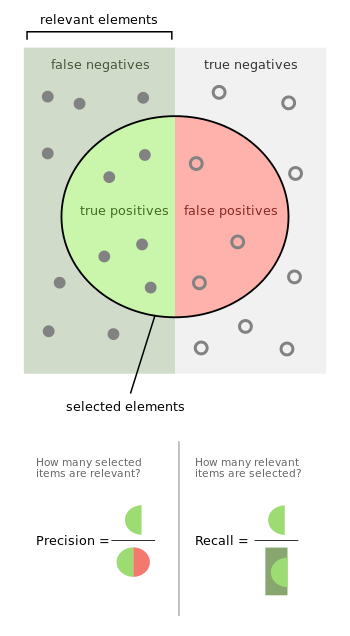
\includegraphics[width=\linewidth]{./figures/precision_recall.png}
	\centering
	\caption{example of precision and recall}
\end{figure}

\section{K-Nearest Neighbors (K-NN)}
\begin{enumerate}
	\item choose the number $K$ of neighbours
	\item take the $K$ nearest neighbours of the new data point, according to the Euclidean distance
	\item among these $K$ neighbours, count the number of data points in each category
	\item assign the new data point to the category where you counted the most neighbours
\end{enumerate}




\section{Support Vector Machine (SVM)}

\section{Kernel SVM}

\section{Naive Bayes}

\section{Decision Tree Classification}

\section{Random Forest Classification}

\section{Evaluating Classification Models Performance}